% Source: graduate-coursework/Research/Intro_to_Agents/handouts/Part4_Planning_Workflow.tex

\documentclass[border=4pt]{standalone}
\usepackage{graphicx}
\usepackage{tikz}
\usepackage{xcolor}
\usetikzlibrary{shapes.geometric, arrows.meta, positioning, calc, fit, backgrounds}

\definecolor{UofSCGarnet}{HTML}{73000A}
\definecolor{UofSCBlack}{HTML}{000000}
\definecolor{UofSCWhite}{HTML}{FFFFFF}
\definecolor{UofSCAtlantic}{HTML}{466A9F}
\definecolor{UofSCCongaree}{HTML}{1F414D}
\definecolor{UofSCHorseshoe}{HTML}{65780B}
\definecolor{UofSCRose}{HTML}{CC2E40}
\definecolor{UofSCDarkGarnet}{HTML}{570008}
\definecolor{UofSC90Black}{HTML}{363636}
\definecolor{UofSC70Black}{HTML}{5C5C5C}
\definecolor{UofSC50Black}{HTML}{A2A2A2}

\tikzset{
    box/.style={
        draw=UofSCBlack,
        fill=#1,
        minimum width=2.5cm,
        minimum height=0.8cm,
        text=UofSCWhite,
        font=\small\bfseries,
        align=center,
        inner sep=4pt
    },
    box/.default=UofSCGarnet,
    lightbox/.style={
        draw=UofSCBlack,
        fill=UofSCWhite,
        minimum width=2.5cm,
        minimum height=0.8cm,
        text=UofSCBlack,
        font=\small,
        align=center,
        inner sep=4pt
    },
    arrow/.style={
        ->,
        >=Stealth,
        thick,
        UofSCBlack
    },
    bigarrow/.style={
        ->,
        >=Stealth,
        line width=1.5pt,
        UofSCGarnet
    },
    phase/.style={
        draw=UofSCBlack,
        fill=#1,
        minimum width=3cm,
        minimum height=1cm,
        text=UofSCWhite,
        font=\bfseries,
        align=center
    },
    phase/.default=UofSCGarnet,
    subphase/.style={
        draw=UofSC70Black,
        fill=UofSCWhite,
        minimum width=2.8cm,
        minimum height=0.6cm,
        text=UofSCBlack,
        font=\scriptsize,
        align=center
    },
    cyclebox/.style={
        draw=UofSCBlack,
        line width=1.5pt,
        fill=#1,
        minimum width=2cm,
        minimum height=1.2cm,
        text=UofSCWhite,
        font=\bfseries,
        align=center
    },
    cyclebox/.default=UofSCGarnet
}

\begin{document}
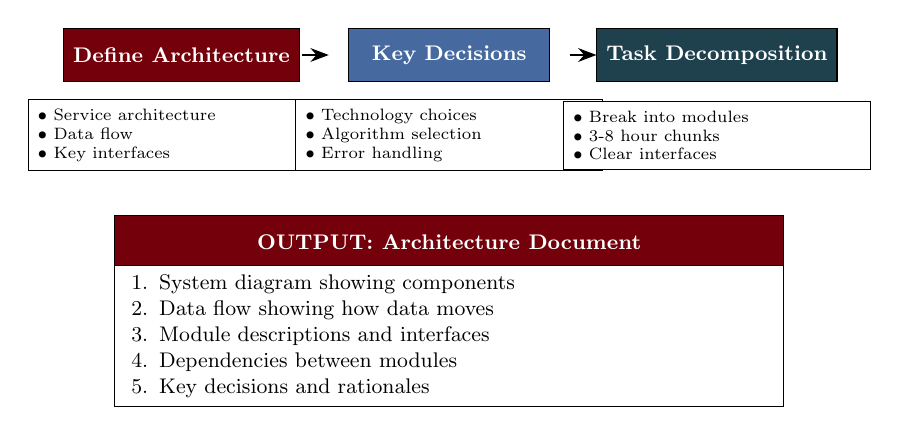
\begin{tikzpicture}[scale=0.85, transform shape]
        % Step boxes
        \node[box=UofSCGarnet, minimum width=3cm] (s1) at (-4,2.5) {Define Architecture};
        \node[lightbox, minimum width=4.5cm, text width=4.3cm, align=left, font=\scriptsize] at (-4,1.3) {
            $\bullet$ Service architecture\\
            $\bullet$ Data flow\\
            $\bullet$ Key interfaces
        };

        \node[box=UofSCAtlantic, minimum width=3cm] (s2) at (0,2.5) {Key Decisions};
        \node[lightbox, minimum width=4.5cm, text width=4.3cm, align=left, font=\scriptsize] at (0,1.3) {
            $\bullet$ Technology choices\\
            $\bullet$ Algorithm selection\\
            $\bullet$ Error handling
        };

        \node[box=UofSCCongaree, minimum width=3cm] (s3) at (4,2.5) {Task Decomposition};
        \node[lightbox, minimum width=4.5cm, text width=4.3cm, align=left, font=\scriptsize] at (4,1.3) {
            $\bullet$ Break into modules\\
            $\bullet$ 3-8 hour chunks\\
            $\bullet$ Clear interfaces
        };

        % Arrows between steps
        \draw[arrow, thick] (-2.2,2.5) -- (-1.8,2.5);
        \draw[arrow, thick] (1.8,2.5) -- (2.2,2.5);

        % Output section
        \node[box=UofSCGarnet, minimum width=10cm, minimum height=0.8cm] at (0,-0.3) {OUTPUT: Architecture Document};
        \node[lightbox, minimum width=10cm, minimum height=1.8cm, text width=9.5cm, align=left] at (0,-1.7) {
            1. System diagram showing components\\
            2. Data flow showing how data moves\\
            3. Module descriptions and interfaces\\
            4. Dependencies between modules\\
            5. Key decisions and rationales
        };
    \end{tikzpicture}
\end{document}
